\chapter{Electrical System}

Readers can find a simplified schematic of Piranha's electrical system in Figure \ref{fig:03overview}. Figure \ref{fig:03test-bench} shows the real-world test bench. 

\begin{figure}[H]
    \centering
    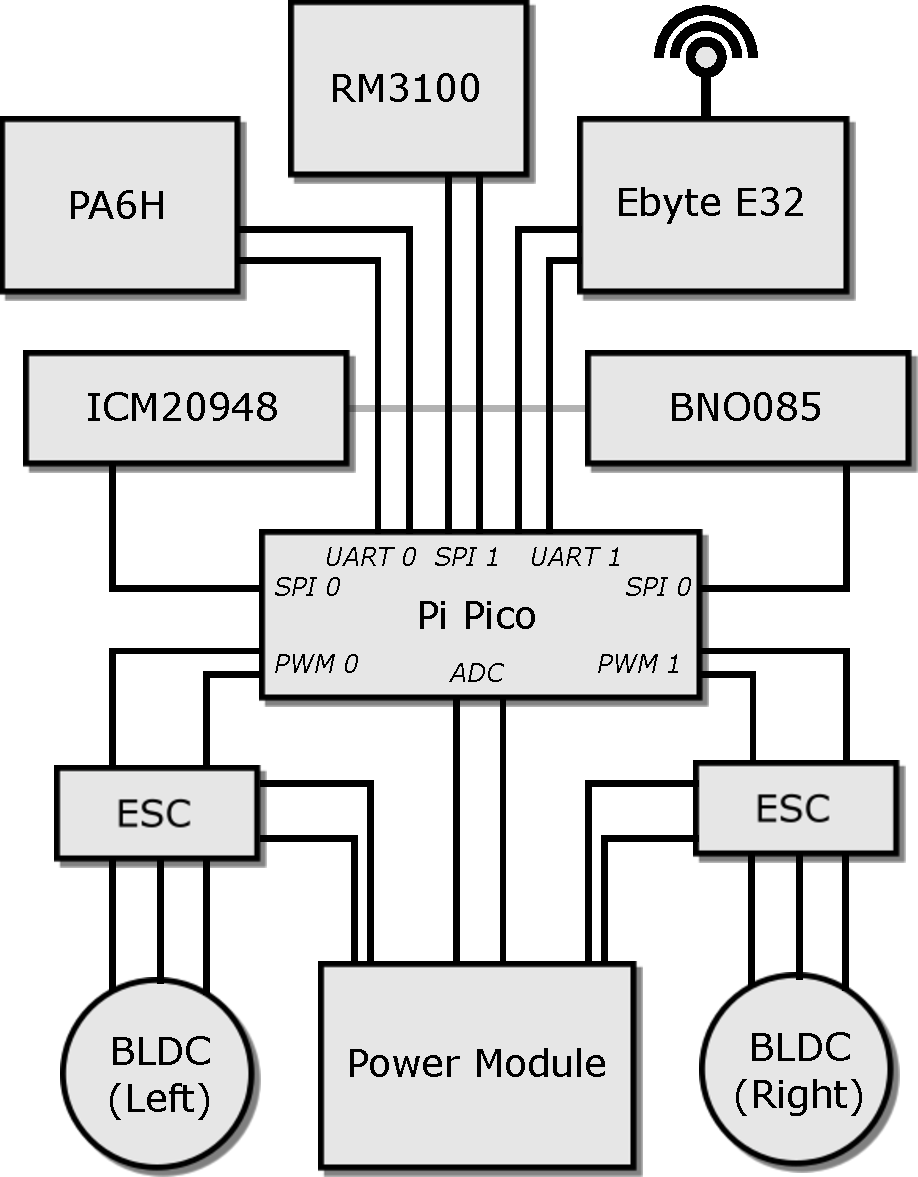
\includegraphics[width=.5\textwidth]{03overview.pdf}
    \caption{The electrical system overview.}
    \label{fig:03overview}
\end{figure}

\begin{figure}[H]
    \centering
    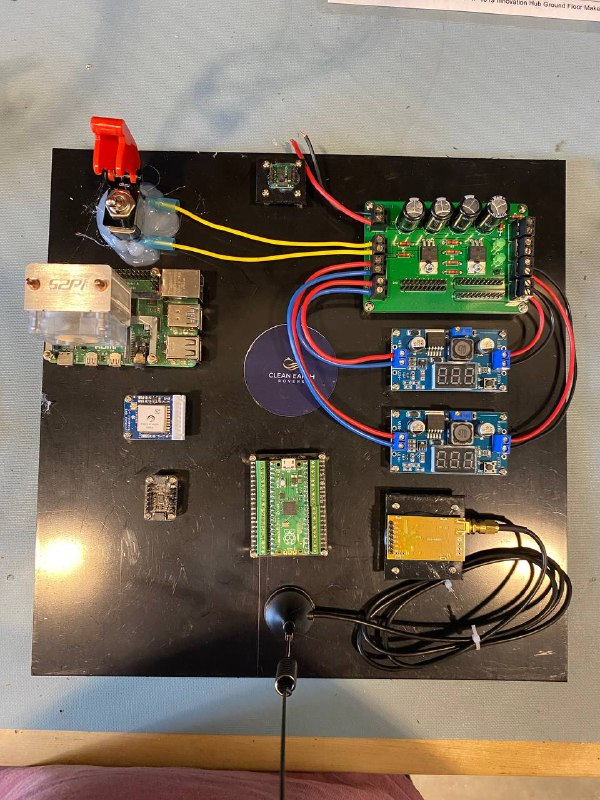
\includegraphics[width=.8\textwidth]{images/03test-bench.jpeg}
    \caption{The figure shows Piranha's test module we built in 1819 Innovation Hub for testing the software functions and electrical design.}
    \label{fig:03test-bench}
\end{figure}

\section{Power Module}

We customized the power module on Piranha to distribute the necessary electrical power to every modules module, including the electrical speed controllers, the Pi Pico, sensors, etc. The board is designed by KiCad and manufactured by JLCPCB. Since the power module carries more than 40-ampere current in the working condition, we covered the PCB with an extra copper layer made by the laser cutter.

The power module also contains several physical switches, including a master switch, two emergency stop switches, and a voltage measurement point for maintenance usage. These switches control the power output to the two thrusters by controlling the gate voltages of two TK4R3E06PL MOSFETs. Table \ref{table:03mosfet} lists its specifications.

The schematic and the rendered 3D model of the Piranha's power module are provided in Figure \ref{fig:03power} and Figure \ref{fig:03shutdown3d}. A PCB prototype board is shown in Figure \ref{fig:03power-pcb}, the electrical components are not soldered yet.

\begin{figure}[H]
    \centering
    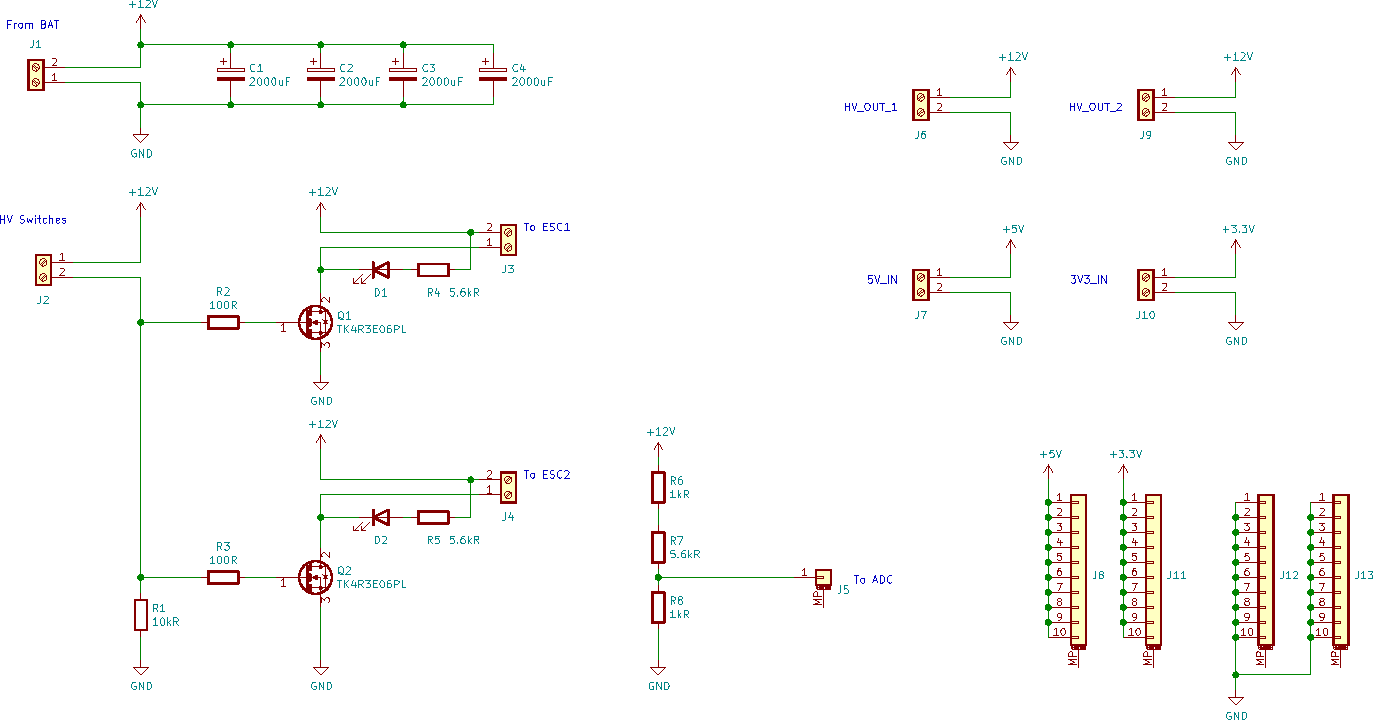
\includegraphics[width=.9\textwidth]{images/03shutdown-sch-no-title.pdf}
    \caption{The overall schematic of the power module.}
    \label{fig:03power}
\end{figure}

\begin{figure}[H]
    \centering
    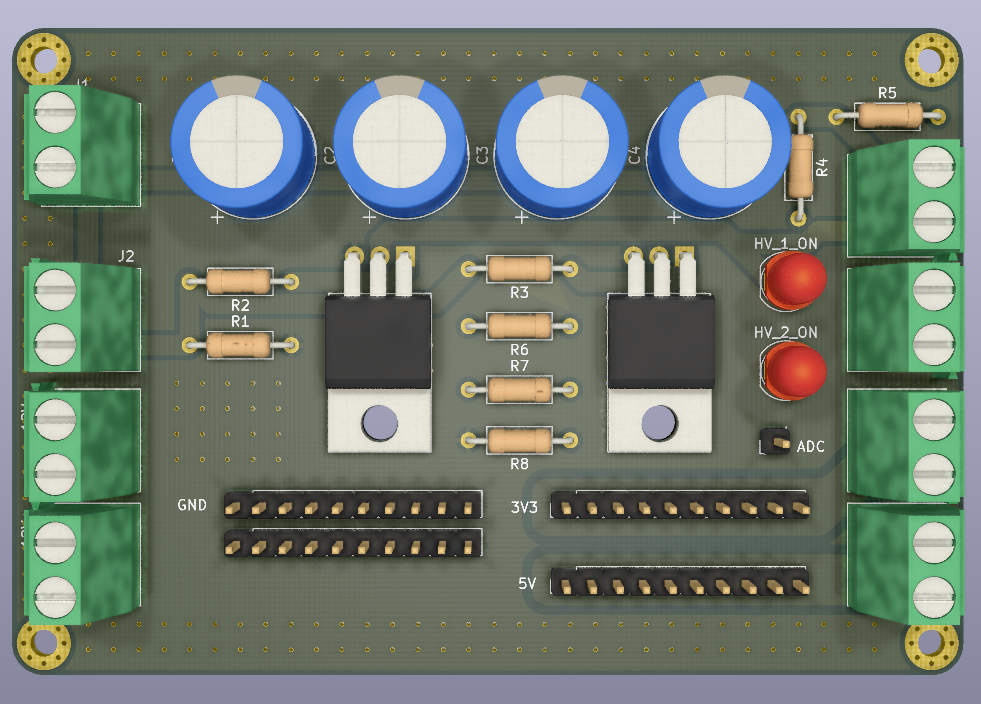
\includegraphics[width=.8\textwidth]{03shutdown3d.png}
    \caption{Power module rendered 3D view in KiCad.}
    \label{fig:03shutdown3d}
\end{figure}

\begin{figure}[H]
    \centering
    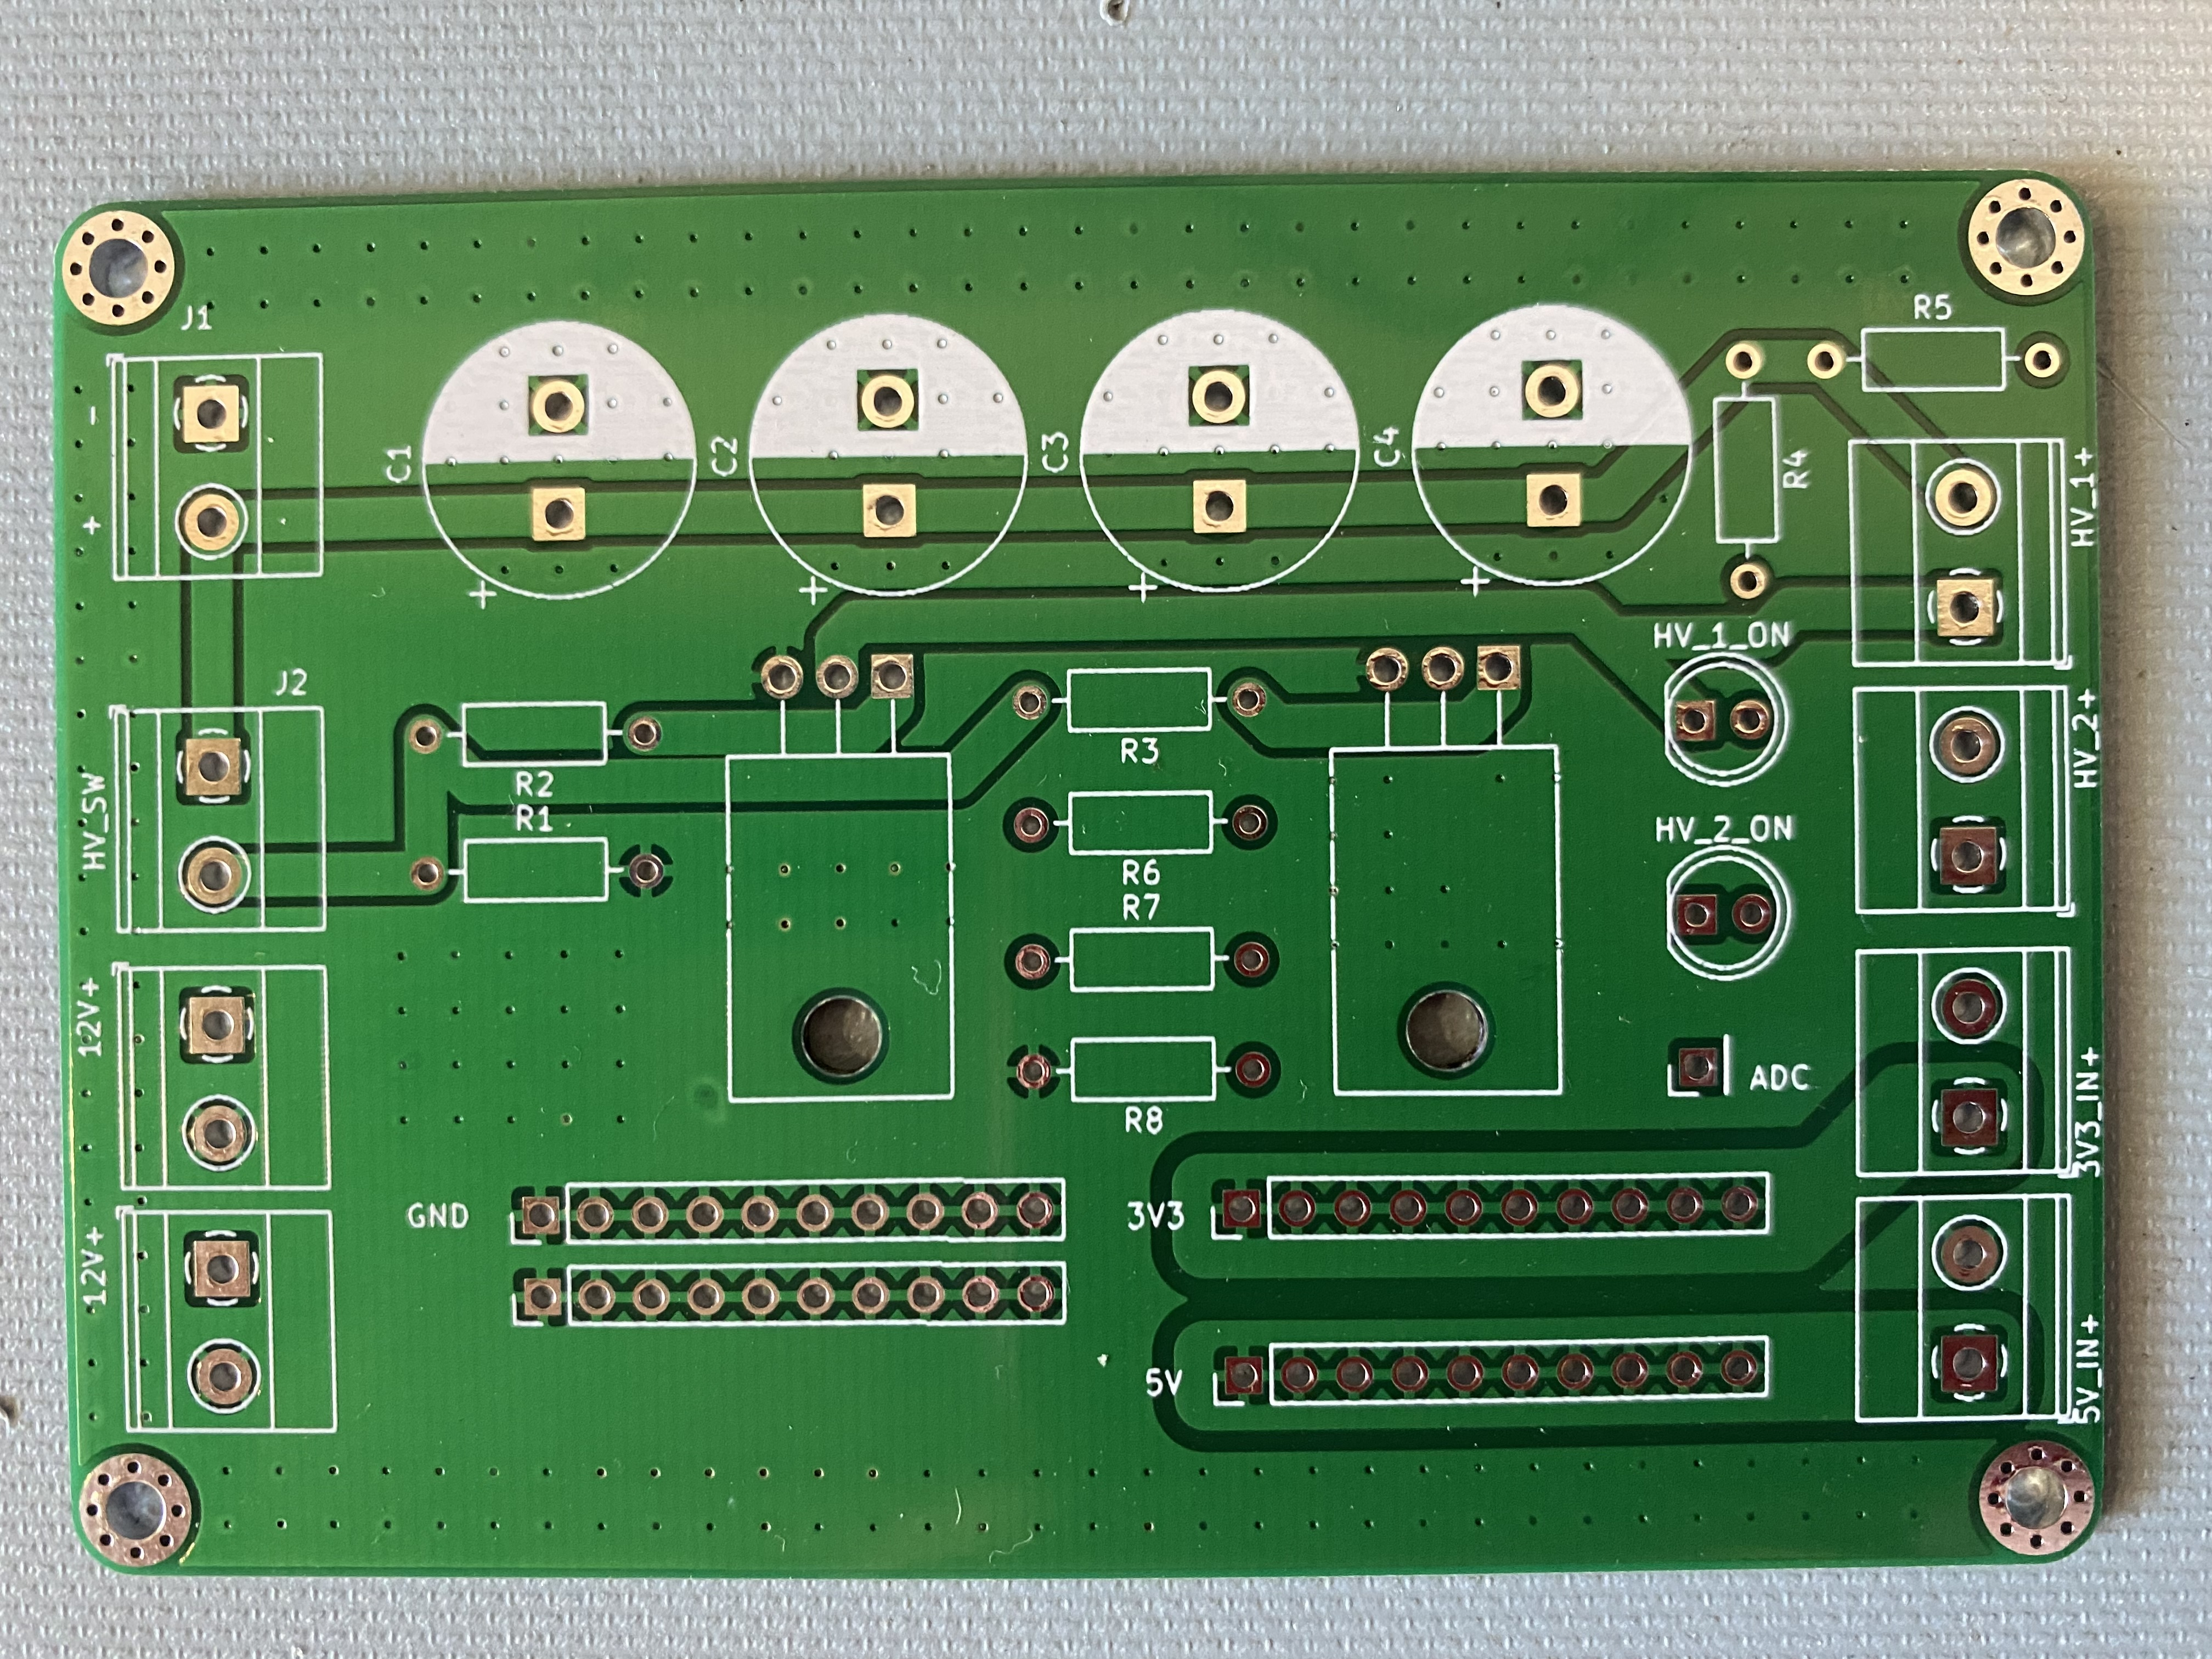
\includegraphics[width=.8\textwidth]{images/03power-module-pcb.JPG}
    \caption{The PCB prototype for the power board manufactured by JLCPCB.}
    \label{fig:03power-pcb}
\end{figure}

Table \ref{table:03powerboard} lists the Piranha's power board specification.

\begin{table}[ht]
\caption{Technical Specifications of the Power Board} % title of Table
\centering % used for centering table
\renewcommand{\arraystretch}{0.8}
\begin{tabular}{l l} % centered columns (4 columns)
\hline
\textbf{Characteristics} & \textbf{Rating} \\ [0.5ex] % inserts table
%heading
\hline % inserts single horizontal line
Maximum input voltage  & $25\ V$ \\
Maximum main output current & $2\times 80\ A$ \\
Maximum working temperature & $125\degree\ C$ \\
Maximum $3.3V$ output current & $3\ A$ \\
Maximum $5V$ output current & $3\ A$ \\
\hline %inserts single line
\end{tabular}
\label{table:03powerboard} % is used to refer this table in the text
\end{table}

Please know that this table only describes the capability of the power board itself. It does not reflect the whole system limitation. For example, the maximum current consumed by a thruster is only $24\ A$.

\subsection{MOSFET}

The power module has two Toshiba TK4R3E06PL MOSFETs as the primary relays. You can find part of its technical specifications in Table \ref{table:03mosfet}. These MOSFETs carry the whole current for the two electrical speed controllers. The external physical switches directly control the voltage on the gates. For safety reasons, no software logic is behind the power control system.

\begin{table}[ht]
\caption{Technical Specifications of TOSHIBA TK4R3E06PL (part)} % title of Table
\centering % used for centering table
\renewcommand{\arraystretch}{0.8}
\begin{tabular}{l c l} % centered columns (4 columns)
\hline
\textbf{Characteristics} & \textbf{Symbol} & \textbf{Rating} \\
%heading
\hline % inserts single horizontal line
Maximum drain-source voltage & $V_{DSS}$ & $60\ V$ \\
Maximum gate-source voltage & $V_{GSS}$ & $20\ V$ \\
Maximum drain current (DC) & $I_D$ & $80\ A$ \\
Maximum channel temperature & $T_{ch}$ & $175\ \degree C$ \\
Channel-to-case thermal resistance (T=$25\ \degree C$) & $R_{th(ch-c)}$  & 1.72\ \degree C/W  \\
Drain-source on-resistance at $V_{GS}=10\ V, I_D = 34\ A$ & $R_{DS(ON)}$ & $3.3{\rm m}\Omega$ (Typical) \\
\hline %inserts single line
\end{tabular}
\label{table:03mosfet} % is used to refer this table in the text
\end{table}

MOSFETs, compared with regular mechanical relays, have huge advantages over the whole life cycle \cite{TK4R3E06PL}. However, due to the characteristics of the PN junction, we need to do some calculations to ensure that, under full workload, the thermal rise of the MOSFETs is within the operational range. 

\subsection{Thermal Estimation}

Because one MOSFET controls only one thruster, the maximum load for each MOSFET approximately equals the full power of the thruster. We ignored the other power consumers like Pi Pico and ESCs since their power ratings are only a few milliwatts. The heat dissipation of the MOSFETs under the maximum workload ($24\ A$), according to Table \ref{table:03mosfet}, can be calculated through Ohm's Law:

\begin{equation}
    P_w=I^2 R_{ds(on)}=24\ A^2 \times 3.3\ {\rm m}\Omega=1.9008\ W
\end{equation}

Given the room temperature $25\degree C$, the maximum junction temperature under full workload is:

\begin{equation}
    T_j=T_r+P_w R_{th(ch-c)}=25\degree C+1.9008\ W\times 1.72C\degree\ C/W=28.269376 \degree C < T_{max} = 175\ \degree C
\end{equation}

Which is well within the temperature range of TK4R3E06PL shown in Table \ref{table:03mosfet}.

\subsection{Switch system}

\subsection{Voltage Measuring Point}

The central control unit can measure the voltage of the battery system through the exposed ADC port on the Piranha's power board. The voltage on the ADC port is divided from the terminal voltage from the battery system by a series of resistors shown in Figure \ref{fig:03voltage-div}.

\begin{figure}[ht]
    \centering
    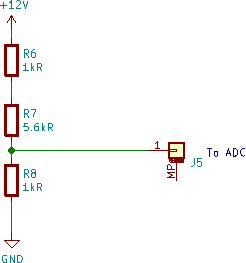
\includegraphics[width=.4\textwidth]{03voltage-div.pdf}
    \caption{The voltage divider circuit. J5 is supposed to connect to the analog input pin of the MCU.}
    \label{fig:03voltage-div}
\end{figure}

One can calculate the voltage ratio by:

\begin{equation}
    H_{ADC}=\frac{R8}{R6+R7+R8}=\frac{1}{7.6}
\end{equation}

\section{Battery System}

Piranha uses two paralleled connected Lithium-ion battery modules from BlueRobotics Inc. Each of them comprises 24 SAMSUNG INR18650-30Q cells, combined in a 4S6P configuration, shown in the Figure \ref{fig:03battery}. Table \ref{table:03battery} lists the technical specification of a single module.

\begin{figure}[ht]
    \centering
    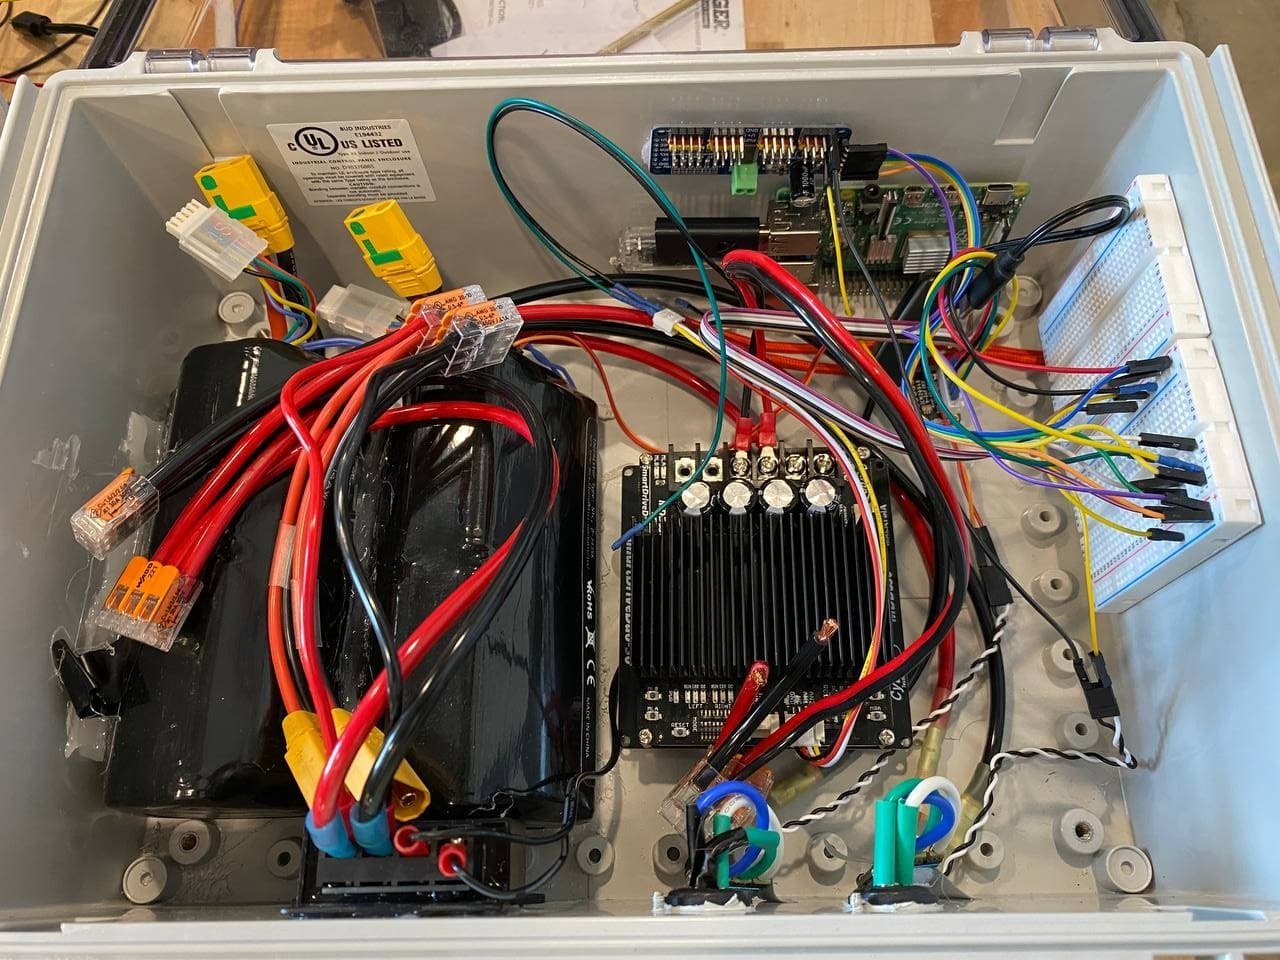
\includegraphics[width=.6\textwidth]{images/03batterysystem.jpg}
    \caption{I took the picture at an early stage test. The battery packs on the left are glued to the box to prevent collisions.}
    \label{fig:03battery}
\end{figure}

\begin{table}[ht]
\caption{Technical Specifications of BlueRobotics Lithium-ion Battery Module ($14.8\ V,\ 18\ Ah$)} % title of Table
\centering % used for centering table
\renewcommand{\arraystretch}{0.8}
\begin{tabular}{l l} % centered columns (4 columns)
\hline
\textbf{Characteristics} & \textbf{Rating} \\ 
%heading
\hline % inserts single horizontal line
Nominal Voltage  & $14.8\ V$ \\
Nominal Capacity & $18.0\ Ah$ \\
Cell Configuration & $4S6P$ \\
Maximum Continuous Current Draw & $90\ A$ \\
\hline %inserts single line
\end{tabular}
\label{table:03battery} % is used to refer this table in the text
\end{table}


\section{Motors (BLDC)}

Piranha equipped two BlueRobotics T200 Thrusters at the rear, shown in Figure \ref{fig:03thruster-test}. By the aerospace terminology convention, these thrusters are called motors in this article. They generate the main propulsion force for the vehicle.

\begin{figure}[ht]
    \centering
    \includegraphics[width=.6\textwidth]{03thruster-test.png}
    \caption{I calibrated two thrusters with a game controller. The right thruster is spinning. Meanwhile, the left one is not moving.}
    \label{fig:03thruster-test}
\end{figure}

Table \ref{table:03motor} lists the technical specifications of the motor.

\begin{table}[ht]
\caption{Technical Specifications of BlueRobotics T200 Thruster (part)} % title of Table
\centering % used for centering table
\renewcommand{\arraystretch}{0.8}
\begin{tabular}{l c l} % centered columns (4 columns)
\hline
\textbf{Characteristics} & \textbf{Rating} \\
%heading
\hline % inserts single horizontal line
Full Throttle FWD/REV Thrust \@ Nominal (16 V) & $5.25\ /\ 4.1\ kgf$ \\
Operating Voltage & $7-20\ V$ \\
Full Throttle Current \@ Nominal (16 V) & $24\ A$ \\
Full Throttle Power \@ Nominal (16 V) & $390\ W$ \\
\hline
\end{tabular}
\label{table:03motor} % is used to refer this table in the text
\end{table}

\section{Electric Speed Controller (ESC)}

The speed controller model is BlueRobotics Basic ESC, shown in Figure \ref{fig:03esc}. The ESCs on Piranha are controlled by two pulse-width modulated signals (PWM) generated by Pi Pico.

\begin{figure}
    \centering
    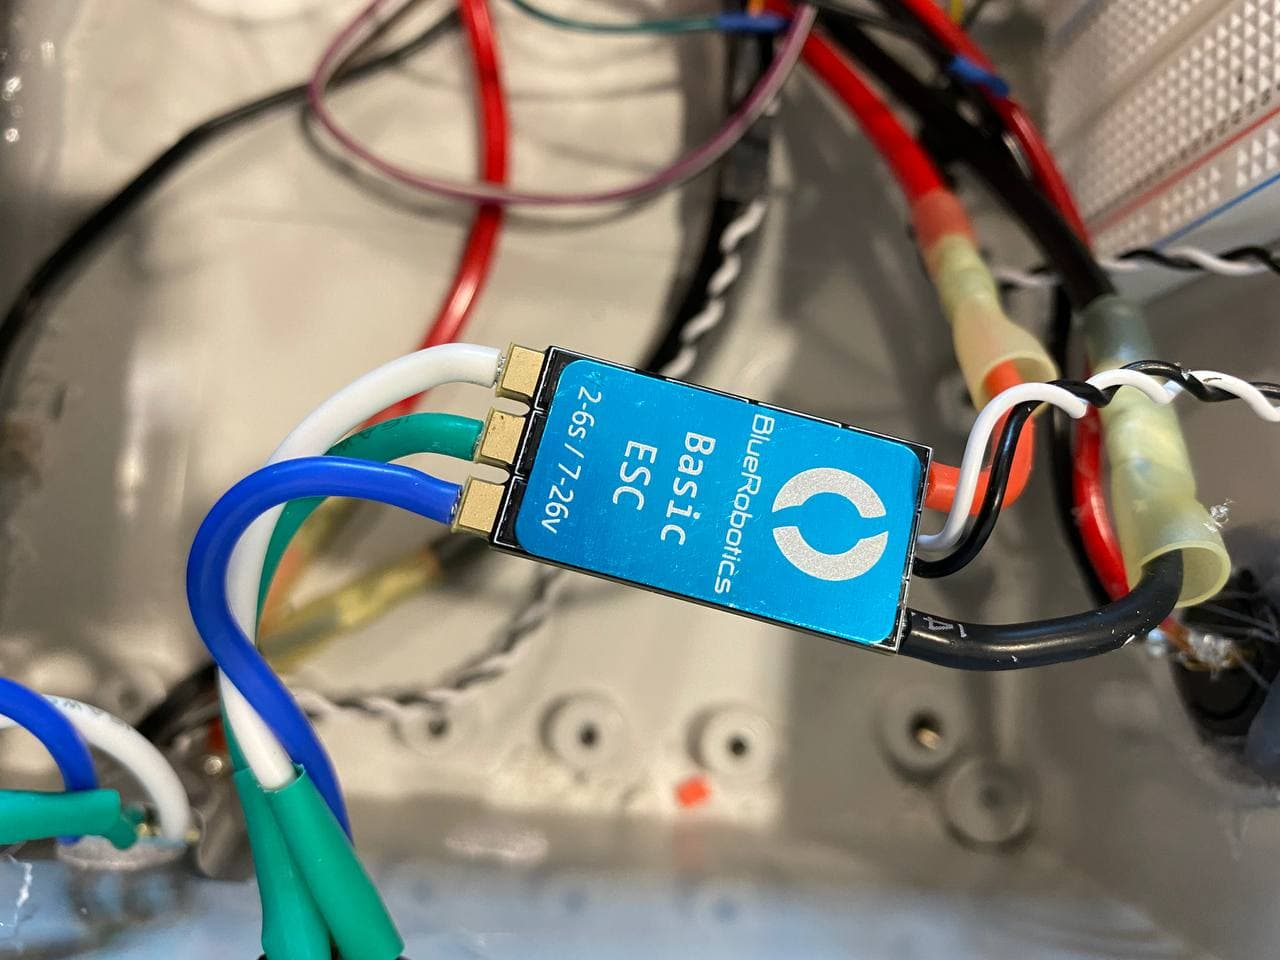
\includegraphics[width=.6\textwidth]{03esc.jpg}
    \caption{BlueRobotics Basic ESC.}
    \label{fig:03esc}
\end{figure}

Table \ref{table:03esc} lists their technical specifications.

\begin{table}[ht]
\caption{Technical Specifications of BlueRobotics Basic ESC (part)} % title of Table
\centering % used for centering table
\renewcommand{\arraystretch}{0.8}
\begin{tabular}{l c l} % centered columns (4 columns)
\hline
\textbf{Characteristics} & \textbf{Rating} \\ 
%heading
\hline % inserts single horizontal line
Operating Voltage & $7-26\ V$ \\
Maximum Current & $30\ A$ \\
Maximum Update Rate & $400\ {\rm Hz}$ \\
Stop Signal Width & $1500\ \mu s$ \\
Maximum Forward Signal Width & $1900\ \mu s$ \\
Maximum Backward Signal Width & $1100\ \mu s$ \\
\hline
\end{tabular}
\label{table:03esc} % is used to refer this table in the text
\end{table}

\section{MCU}

The microcontroller unit, also known as MCU, is the Pi Pico, designed and manufactured by Pi Foundation, shown in Figure \ref{fig:03pico}. Its specification can be found in Table \ref{table:03pico}.

\begin{figure}
    \centering
    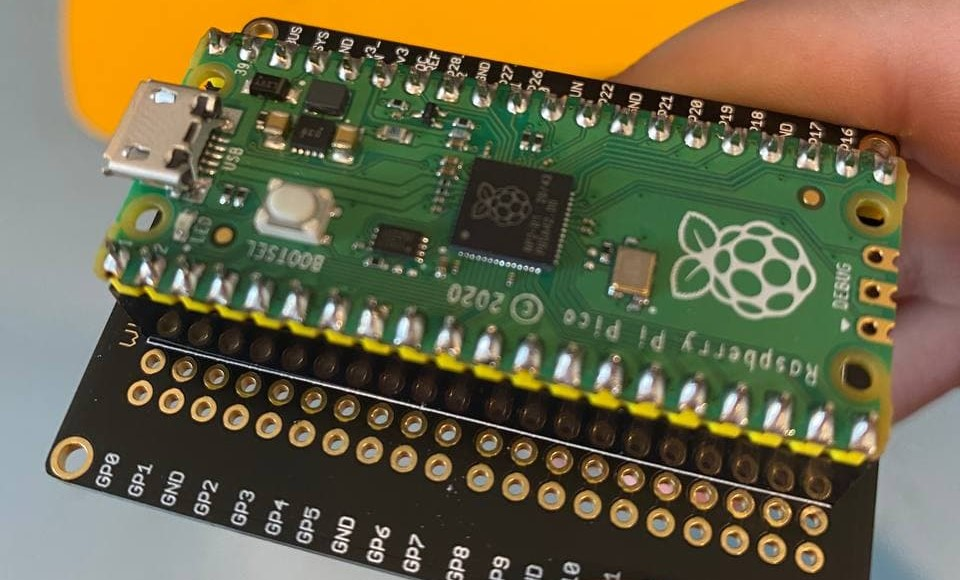
\includegraphics[width=.6\textwidth]{03pico.jpg}
    \caption{Pi Pico installed on the breakout board.}
    \label{fig:03pico}
\end{figure}

The chip model on the Pi Pico board is RP2040. It has a dual-core cortex M0+ at up to 133MHz frequency. For its specification, please refer to the extra document files.

\begin{table}[ht]
\caption{Electrical Specifications of Pi Pico (part)} % title of Table
\centering % used for centering table
\renewcommand{\arraystretch}{0.8}
\begin{tabular}{l c l} % centered columns (4 columns)
\hline
\textbf{Characteristics} & \textbf{Rating} \\ 
%heading
\hline % inserts single horizontal line
Supply Voltage & $1.8-5.5V$ \\
Operating Temperature & $-20 - 85\ \degree C$ \\
VBUS Current & $1.2-92.8\ mA$ \\
Flash Size & $2\ {\rm MByte}$ \\
\hline
\end{tabular}
\label{table:03pico} % is used to refer this table in the text
\end{table}

\section{IMU}

On Piranha, there are two IMUs. One is Adafruit TDK InvenSense ICM-20948 9-DoF shown as in Figure \ref{fig:03icm20948}, the other is Ceva BNO085 IMU, shown in Figure \ref{fig:03bno085}.  

ICM-20948 is the latest 9-axis MotionTracking device designed by TDK. It contains a 3-axis MEMS accelerometer, a 3-axis MEMS gyroscope, and a 3-axis MEMS magnetometer. It also has a built-in temperature sensor that can compensate for the error caused by the temperature shifting. The specification of ICM-20948 can be found in Table \ref{table:03icm20948}. ICM20948 features a built-in digital motion processor to process the acceleration data on the chip, so the Pi Pico can directly access the real-time position and speed data.

BNO085 is co-designed by Ceva and Bosch. Like ICM20948, it also integrates a triaxial accelerometer, a triaxial gyroscope, a magnetometer, and a 32-bit ARM® Cortex™-M0+ microcontroller running CEVA's SH-2 firmware that can output the integrated position result directly. Its specification can be found in Table \ref{table:03bno085}.

\begin{figure}[H]
    \centering
    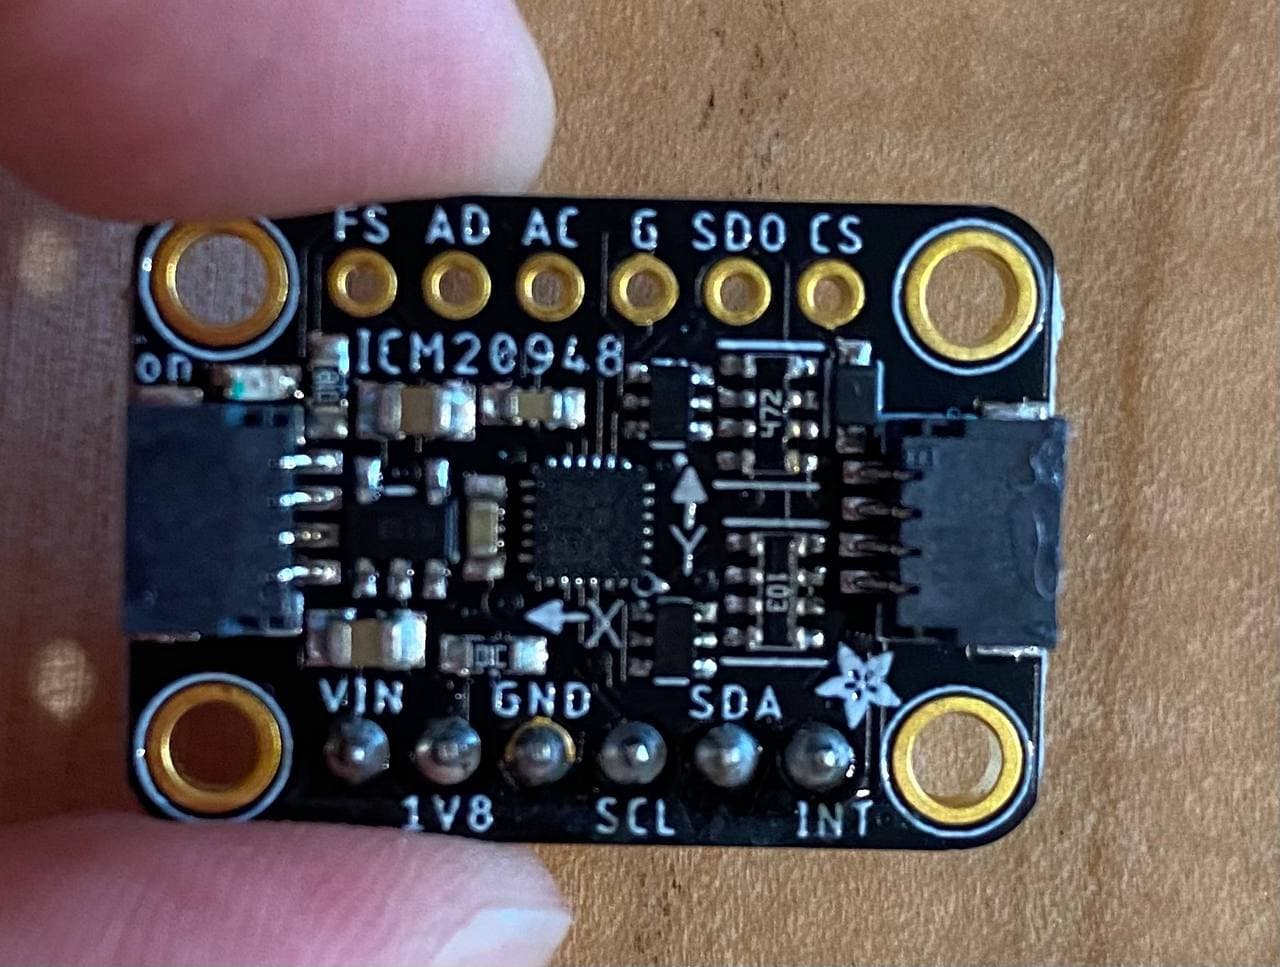
\includegraphics[width=.6\textwidth]{images/03icm20948.jpg}
    \caption{Adafruit TDK InvenSense ICM-20948 9-DoF IMU.}
    \label{fig:03icm20948}
\end{figure}

\begin{figure}[H]
    \centering
    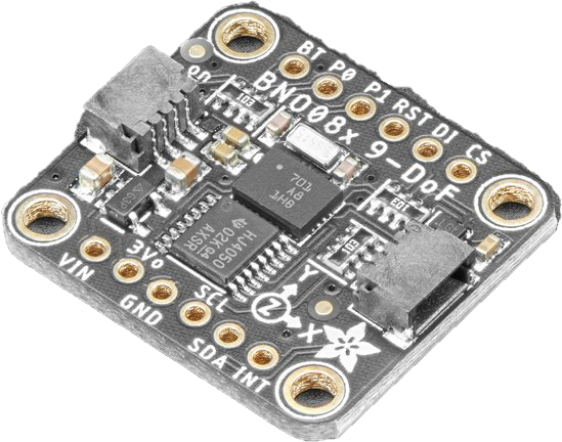
\includegraphics[width=.6\textwidth]{images/03bno085.png}
    \caption{Adafruit 9-DOF Orientation IMU Fusion Breakout - BNO085.}
    \label{fig:03bno085}
\end{figure}


\begin{table}[H]
\caption{Specification of ICM-20948 (part)} % title of Table
\centering % used for centering table
\renewcommand{\arraystretch}{0.8}
\begin{tabular}{l c l} % centered columns (4 columns)
\hline
\textbf{Characteristics} & \textbf{Rating} \\ 
%heading
\hline % inserts single horizontal line
Gyroscope Date Rate (Low Pass Filter On)& $1.125\ {\rm kHz}$ \\
Accelerometer Date Rate (Low Pass Filter On) & $1.125\ {\rm kHz}$ \\
Magnetometer Date Rate & $100\ {\rm Hz}$ \\
Gyroscope Full-Scale Range (GYRO\_FS\_SEL=0) & $\pm 250\ dps$ \\
Accelerometer Full-Scale Range (ACCEL\_FS=0) & $\pm 2\ G$ \\
Magnetometer Full-Scale Range & $\pm 4900\ \mu T$ \\

\hline
\end{tabular}
\label{table:03icm20948} % is used to refer this table in the text
\end{table}

\begin{table}[H]
\caption{Specification of BNO-085 (part)} % title of Table
\centering % used for centering table
\renewcommand{\arraystretch}{0.8}
\begin{tabular}{l c l} % centered columns (4 columns)
\hline
\textbf{Characteristics} & \textbf{Rating} \\ 
%heading
\hline % inserts single horizontal line
Gyroscope Date Rate (Low Pass Filter On)& $1\ {\rm kHz}$ \\
Accelerometer Date Rate (Low Pass Filter On) & $0.5\ {\rm kHz}$ \\
Magnetometer Date Rate & $100\ {\rm Hz}$ \\
Gyroscope Full-Scale Range (GYRO\_FS\_SEL=0) & $\pm 2000\ dps$ \\
Accelerometer Full-Scale Range (ACCEL\_FS=0) & $\pm 8\ G$ \\

\hline
\end{tabular}
\label{table:03bno085} % is used to refer this table in the text
\end{table}


\section{Magnetometer}

Since electromagnetic interference can easily disrupt magnetometer readings, Piranha also has a dedicated magnetometer, RM3100, installed away from the motors, batteries, and other electrical components. The RM3100 sensor is shown in Figure \ref{fig:03rm3100}, its technical specification is listed in Table \ref{table:03rm3100}.

\begin{figure}[ht]
    \centering
    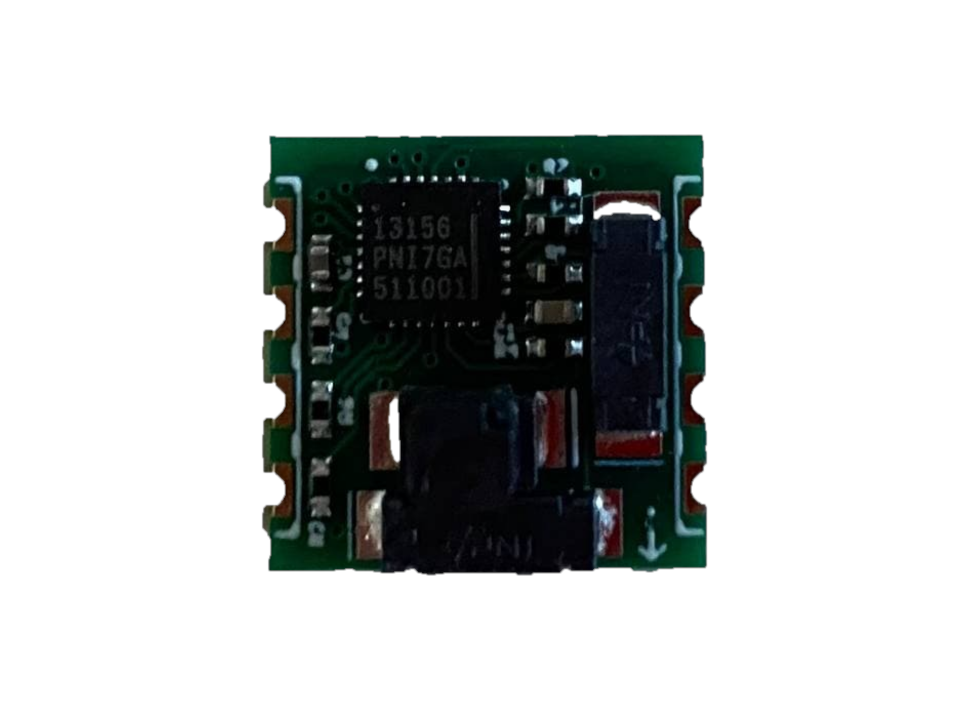
\includegraphics[width=.6\textwidth]{images/03rm3100.png}
    \caption{WitMotion High-Precision RM3100 Magnetometer Sensor}
    \label{fig:03rm3100}
\end{figure}

\begin{table}[ht]
\caption{Specifications of RM3100 (part)} % title of Table
\centering % used for centering table
\renewcommand{\arraystretch}{0.8}
\begin{tabular}{l c l} % centered columns (4 columns)
\hline
\textbf{Characteristics} & \textbf{Rating} \\ 
%heading
\hline % inserts single horizontal line
Maximum Single-Axis Sample Rate & 1600/850/440 Hz \\
DC Supply Voltage & $2.0\sim3.6$ V \\
Field Measurement Range & $-800 \sim 800\ m\mu$T \\
Sensitivity & 50/26/13 nT \\
Noise & 30/20/15 \\
\hline
\end{tabular}
\label{table:03rm3100} % is used to refer this table in the text
\end{table}

One must verify that sensitivity of the magnetometer measurement is high enough to detect the earth's magnetic field, which is approximately 0.6 Gauss (48A/m; 6000 nT), before using it. RM3100 has a measurement range within $\pm 800\ \mu$T or $\pm 8\times 10^5\ n$T, which is well more significant than the earth's magnetic field strength, and high sensitivity as low as $\pm 13\ n$T which is only $0.21\%$ of the earth's magnetic field strength. So it is reasonable to use RM3100 as a digital compass on Piranha.

In applications like small fixed-wing planes and rotors, the engineers often consider magnetometer readings very noisy because the electromagnetic interference is usually very high. However, on Piranha, because the magnetometer is put far from the interference source, we believe the data to be reliable and put more weight on them in the sensor fusion (EKF) part. This report will explain it later.

\section{GPS}

GPS is essential in the position estimation process because it provides drift-free position and speed data in real-time.

On Piranha, the GPS module is Adafruit Ultimate GPS, built around the MTK3339 chipset. Readers can find its technical specifications in Table \ref{table:03gps}.

\begin{table}[ht]
\caption{Specification of Adafruit Ultimate GPS (part)} % title of Table
\centering % used for centering table
\renewcommand{\arraystretch}{0.8}
\begin{tabular}{l c l} % centered columns (4 columns)
\hline
\textbf{Characteristics} & \textbf{Rating} \\ 
%heading
\hline % inserts single horizontal line
Satellites & 22 tracking, 66 searching \\
Update Rate & $1-10 {\rm Hz}$ \\
Position Accuracy & $<3 \ m$ \\
Velocity Accuracy & $<0.1\ m/s$ \\
Maximum Velocity & $515\ m/s$ \\

\hline
\end{tabular}
\label{table:03gps} % is used to refer this table in the text
\end{table}

\section{Wireless Module}

We designed Piranha with a manual mode, which allows the human operator to control the boat from a distance. During the development, we considered multiple different communication methods and tested them all. Table \ref{table:03wireless} shows the comparison among them.

\begin{table}[H]
\caption{Wireless Communication Method Comparison} % title of Table
\centering % used for centering table
\renewcommand{\arraystretch}{0.8}
\begin{tabular}{l l l l l} % centered columns (4 columns)
\hline
\textbf{Method} & \textbf{Speed} & \textbf{Range} & \textbf{Cost} & \textbf{Power Consumption} \\ 

%heading
\hline % inserts single horizontal line
4G/LTE & 100 Mbps & Depends on the coverage & High\footnotemark & $~100\ {\rm mW}$ \\
WiFi & 150 Mbps & $< 70\ {\rm ft}$ & Low & $~100\ {\rm mW}$ \\
RF Radio & 10 Mbps & $\sim 1\ {\rm mile}$ & High & $\sim 1\ {\rm W}$ \\
LoRa & $0.3- 20 {\rm kbps}$ & $\sim 5\ {\rm miles}$ & Low & $\sim 1\ {\rm W}$ \\
\hline
\end{tabular}
\label{table:03wireless} % is used to refer this table in the text
\end{table}

\footnotetext{Most 4G plans in the U.S. need a monthly payment.}

Piranha is a water surface robot, so its moving range depends on the control signal range if controlled by a human operator. For this reason, the control signal range should be as long as possible. Since the control signal only has simple commands, it does not need high bandwidth to work.

As a result, We chose to use LoRa on Piranha as the main wireless communication method from the ground station. LoRa is a wireless communication protocol based on the spread spectrum technology. It is designed for low power, and long-range data transmission \cite{8075570}. The LoRa module on Piranha is the Ebyte E32-915T30D model, shown in Figure \ref{fig:03e32}, it works on the $915 {\rm MHz}$ band. Because it works on an unlicensed band in the U.S., there is no need to get a commercial license from FCC. Its technical specification can be found in Table \ref{table:03e32}.

\begin{figure}
    \centering
    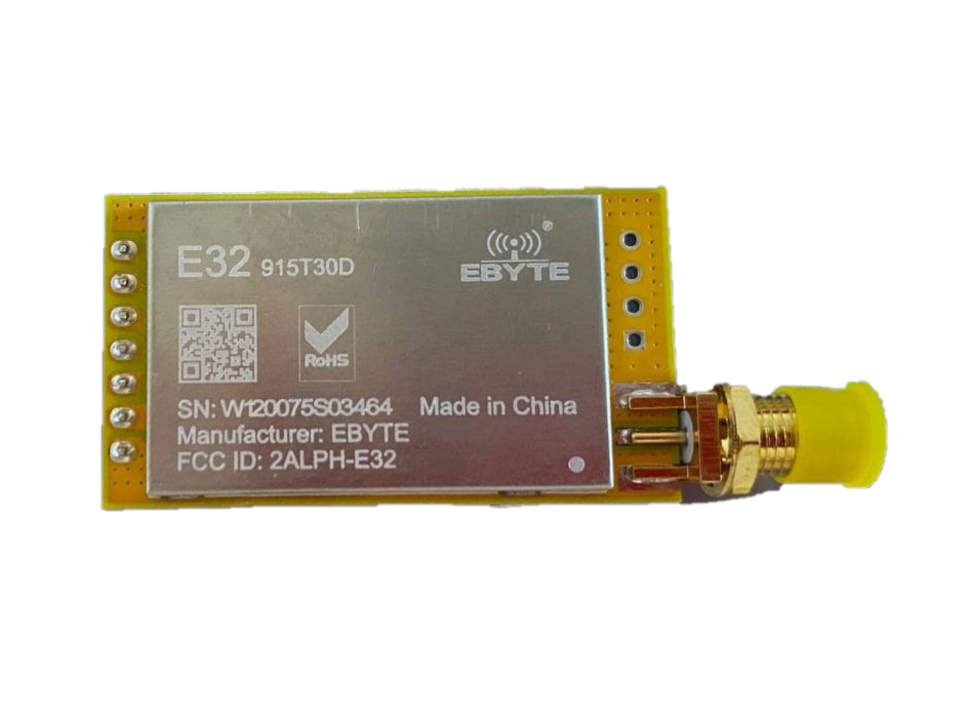
\includegraphics[width=.6\textwidth]{images/03e32.png}
    \caption{E32-915T30D}
    \label{fig:03e32}
\end{figure}

\begin{table}[H]
\caption{Specifications of E32-915T30D} % title of Table
\centering % used for centering table
\renewcommand{\arraystretch}{0.8}
\begin{tabular}{l l l l l} % centered columns (4 columns)
\hline
\textbf{Characteristics} & \textbf{Rating} \\ 
%heading
\hline % inserts single horizontal line
Maximum Transmission Power & $1\ {\rm W}$ \\
Maximum Communication Distance & $8\ {\rm km}$ \\
Air Date Rate & $0.3-19.2$ kbps \\
Maximum Tx Power & $30\ {\rm dBm}$ \\
Maximum Rx Power & $-147\ {\rm dBm}$ \\
\hline
\end{tabular}
\label{table:03e32} % is used to refer this table in the text
\end{table}